\documentclass[11pt,a4paper,oneside]{article}
\usepackage[a4paper,top=2cm,bottom=2.5cm,left=2.5cm,right=2cm]{geometry}
\usepackage[T1]{fontenc}
\usepackage[utf8]{inputenc}
\usepackage[english]{babel}
%\usepackage{frontespizio}
\usepackage{graphicx}
\usepackage{subfig}
\usepackage[english]{varioref}

\begin{document}

%opzione per doppio interlinea
\baselineskip 22pt


%Indice%
\tableofcontents\thispagestyle{empty}\clearpage

\section{Introduction}
\pagenumbering{arabic}
\baselineskip 12pt

\section{The dataset}


\section{Task 1: Related works}

\clearpage

\section{Task 2: From Scratch CNN}
We developed different models of neural networks to work with the given dataset from scratch and we did different test to find the better hyperparameters to build the final model. This section is divided in three parts: in the first one we describe the main preprocessing applied to the data before the training of the models. Then we show how we built a model for classifying the dataset images between \textit{mass} abnormality and \textit{calfication} abnormality. In the last part, we describe the model built to classify between \textit{benign} and \textit{malignant} abnormality.

\subsection{Data Preprocessing}
Starting from the numpy arrays of the dataset images we were given, first of all we deleted all the samples associated with the \textit{baseline patch} label. Since this labeled images were placed in the even positions of the dataset, we just selected all the odd-index samples al discard the others. This is done both for the training data and the test data. \\
Then we aggregated the labels according to the classification that we needed to do: in the $Task\ 2.1$ the classes \textit{mass benign} and  \textit{mass malignant} were aggregated in a unique class \textit{mass}, and so for the \textit{calcification} classes. On the other hand, in the $Task\ 2.2$ we aggregated  \textit{mass benign} and  \textit{cacification benign} in the \textit{benign} class, and the other labels in the \textit{malignant} class.

\begin{figure}[h]
\centering
	\subfloat[][$Task\ 2.1$: 0 for \textit{mass}, 1 for \textit{calcification} \label{fig:label_mass_calc}]
		{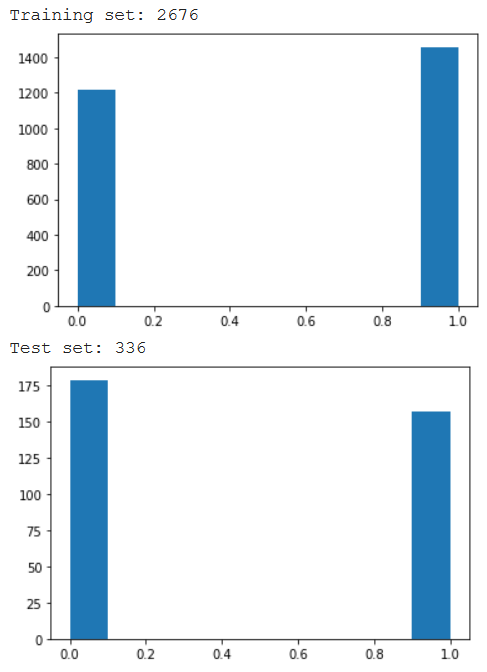
\includegraphics[width=.3\textwidth]{images/label_mass_calc}} \quad
	\subfloat[][$Task\ 2.2$: 0 for \textit{benign}, 1 for \textit{malignant} \label{fig:label_benign_malign}]
		{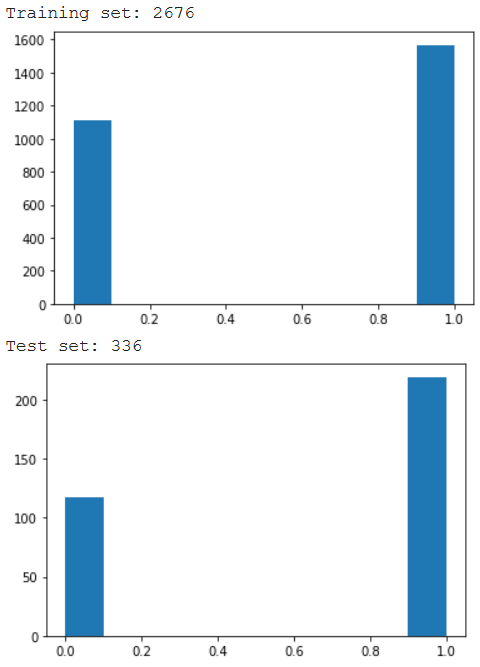
\includegraphics[width=.3\textwidth]{images/label_benign_malign}} \\
\caption{Label distribution}
\label{fig:label distribution}
\end{figure}

For the first case, we can see from the figure that the labels are pretty much equally distributed. Instead, in the second case the dataset is a little more unbalanced towards the \textit{benign} class. \\
Finally, we reshaped all the training images tensors in a single \textit{numpy} array, that has been then normalized. The same has been done for the test images. With regards to the labels, they has been categorizated so that is possible to use the categorical loss function in the model.

\subsection{Task 2.1: Mass-Calcification discriminator}
We first tried to build a simple CNN, with some convolutional and max-pooling layers, and two final dense layers. We trained and tested the model several times, changing the hyperparameters to find a good model for out problem. The final architecture that has been used for the most relevant tests is shown in figure~\ref{fig:scratch_model}. It is made of five convolutional layers, with an increasing number of kernels. Each layer is followed by a max-pooling of $2x2$, except for the last one so that the input of the dense layer is not too reduced. The activation function used in the layers is \textit{ReLu}.

\begin{figure}[h]
\centering
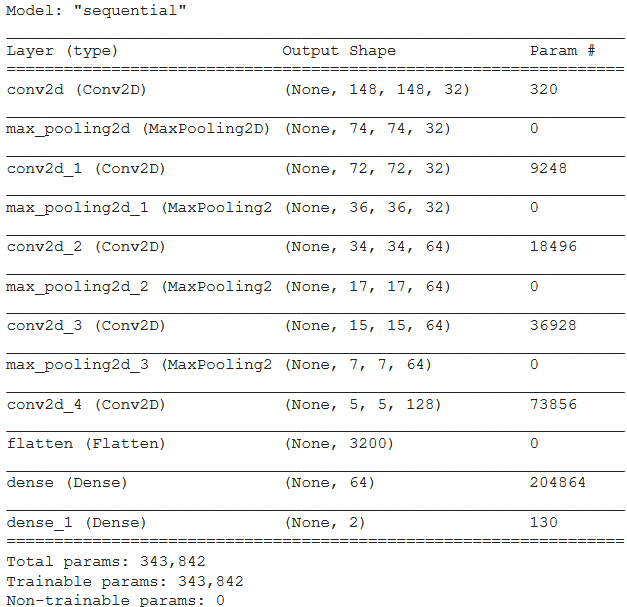
\includegraphics[width=.5\textwidth]{images/scratch_model}
\caption{First model of the CNN from scratch}
\label{fig:scratch_model}
\end{figure}

After asserting the architecture, the model has been trained with different numbers of \textit{hidden units} for the first fully connected layer, but also for different \textit{batch sizes} and different \textit{output functions}. 
In all the tests, the conclusion has been that the network was over-training, and this is the reason for which we have developed a second model, adding a data augmentation preprocessing. 
In the figure~\ref{fig:scratch_accuracy}, we present the results in term of accuracy and loss, but also the consufion matrix (fig.~\ref{fig:scratch_matrix}), related to a test of the model with $512$ hidden units, a batch size of $50$, and the \textit{softmax} function for the output layer. 
The used optimizer is Adam, with the deafult learning rate of $0.001$. As we said before, the gap between the training and validation graphs show that the model is over-training: even if the predictions on the test set are accurate, we cannot rely on this network as it is.
\begin{verbatim}
        network.compile(optimizer='adam',
                loss='categorical_crossentropy',
                metrics=['accuracy'])

        network.fit(train_images, train_labels, epochs=100, batch_size=50, 
                validation_split=0.2, shuffle=True, callbacks=[callback])
\end{verbatim}
\begin{figure}[hb]
\centering
	\begin{minipage}[c]{.4\textwidth}
		\centering\setlength{\captionmargin}{0pt}%
		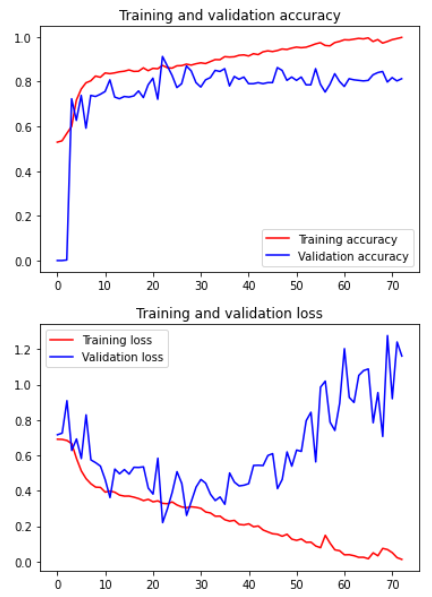
\includegraphics[width=.9\textwidth]{images/scratch_accuracy}
		\caption{Accuracy and loss graphs for the first model training}
		\label{fig:scratch_accuracy}
	\end{minipage}
	\hspace{5mm}%
	\begin{minipage}[c]{.4\textwidth}
		\centering\setlength{\captionmargin}{0pt}%
		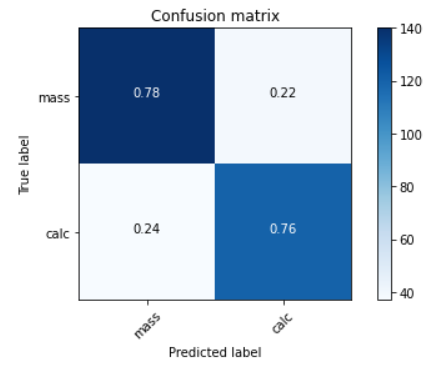
\includegraphics[width=.9\textwidth]{images/scratch_matrix}
		\caption{Normalized confusion matrix for the test set predictions}
		\label{fig:scratch_matrix}
	\end{minipage}%
\end{figure}

\subsubsection{Data augmentation}
To overcome the problem of over-fitting, we augmented our training using the \textit{ImageDataGenerator} class of \textit{keras}. The main variations we adopted were random rotation up to 40 degrees, random vertical and horizontal shifts with a range of 0.2, random zoom with a range of 0.2, random shear with a range of 0.2 and nearest fill model. To set these parameters we referred to the data in the papers we studied in the initial phase of the project. Before applying these variations to the train set, we splitted it to get the validation set separately.

\begin{verbatim}
        train_set, val_set, train_classes, val_classes = 
                train_test_split( train_images, train_labels, test_size=0.2)
        
        train_datagen = ImageDataGenerator(
                rotation_range=40,
                width_shift_range=0.2,
                height_shift_range=0.2,
                shear_range=20,
                zoom_range=0.2,
                horizontal_flip=True,
                fill_mode='nearest')

        train_generator = train_datagen.flow(train_set,train_classes,batch_size=50)
\end{verbatim}

We trained again our model with the augmented training set and with the validation set, and the results were more satisfying, having a mean accuracy around $80\%$. At this point, we wanted to have a more accurate analysis on some hyperparameters so we did several tests changing their values to get a model as good as possible. 

\clearpage

\subsection{Task 2.2: Benign-Malignant discriminator}


\section{Task 3: Pretrained network}


\section{Task 4: Baseline patches}


\section{Task 5: Ensemble network}

\end{document}
